\subsubsection{Information}
\begin{itemize}
	\item \textbf{Course Name:} \href{https://www.coursera.org/learn/ux-design-jobs}{Design a User Experience for Social Good \& Prepare for Jobs}
	\item \textbf{Instructor:} \href{https://www.coursera.org/instructor/google-career-certificates}{Google Career Certificates}
	\item \textbf{Level:} Beginner
	\item \textbf{Enrolled on:} July 24, 2024
	\item \textbf{Finished on:} August 16, 2024
	\item \textbf{Grade Achieved:} 92.85\%
\end{itemize}

\subsubsection{Course is done}
\begin{figure}[!ht]
	\centering
	\begin{subfigure}{0.75\textwidth}
		\centering
		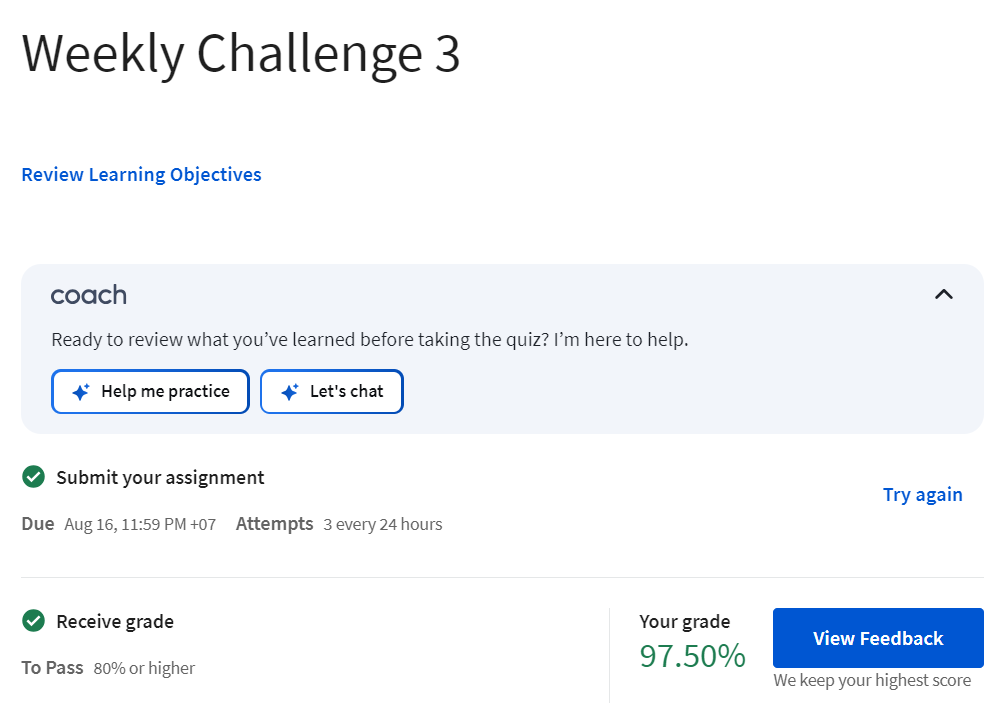
\includegraphics[width=\textwidth]{imgs/Course7-M3.png}
	\end{subfigure}
	\hfill
	\begin{subfigure}{0.75\textwidth}
		\centering
		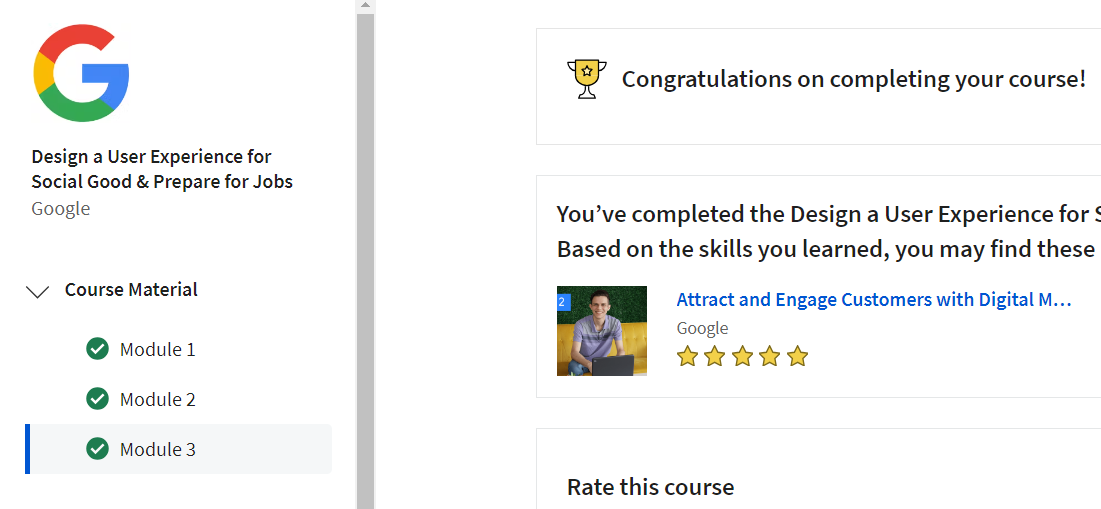
\includegraphics[width=\textwidth]{imgs/Course7-Done.png}
	\end{subfigure}
	\caption{Course 7 - Done}
\end{figure}

\subsubsection{Summary}
\begin{flushleft}
	What I have learned after completing this course:
	\begin{itemize}
		\item Apply each step of the UX design thinking framework (empathize, define, ideate, prototype, test) to create a  project focused on social good.
		\item Build wireframes, mockups, and low-fidelity and high-fidelity prototypes for a dedicated mobile app and a responsive website.
		\item Prepare to successfully interview for an entry-level UX design job.
		\item Determine if freelance design work is a good career fit.
	\end{itemize}
\end{flushleft}

\subsubsection{Details}
\begin{flushleft}
	\begin{description}
		\item[Module 1:] Design for social good and strengthen your portfolio
		      \begin{itemize}
			      \item I have designed a dedicated mobile app and a responsive website focused on social good that showcases everything I've learned in the program.
		      \end{itemize}
		\item[Module 2:] Build a professional presence
		      \begin{itemize}
			      \item I have created a portfolio to showcase my upcoming work.
			      \item I have also learnt about the importance of having a personal brand and building an online presence.
		      \end{itemize}
		\item[Module 3:] Finding a UX job
		      \begin{itemize}
			      \item I have made final adjustments to my portfolio to ensure it's ready to share in job applications.
			      \item I have examined the UX design interview process and develop strategies to succeed in various types of interview.
		      \end{itemize}
	\end{description}
\end{flushleft}